%%%%%%%%%%%%%%%%%%%%%%%%%%%%%%%%%%%%%%%%%
%
% CMPT 424N 111
% Fall Semester
% Lab 5
%
%%%%%%%%%%%%%%%%%%%%%%%%%%%%%%%%%%%%%%%%%

%%%%%%%%%%%%%%%%%%%%%%%%%%%%%%%%%%%%%%%%%
% Short Sectioned Assignment
% LaTeX Template
% Version 1.0 (5/5/12)
%
% This template has been downloaded from: http://www.LaTeXTemplates.com
% Original author: % Frits Wenneker (http://www.howtotex.com)
% License: CC BY-NC-SA 3.0 (http://creativecommons.org/licenses/by-nc-sa/3.0/)
% Modified by Alan G. Labouseur  - alan@labouseur.com
%
%%%%%%%%%%%%%%%%%%%%%%%%%%%%%%%%%%%%%%%%%

%----------------------------------------------------------------------------------------
%	PACKAGES AND OTHER DOCUMENT CONFIGURATIONS
%----------------------------------------------------------------------------------------

\documentclass[letterpaper, 10pt,DIV=13]{scrartcl} 

\usepackage[T1]{fontenc} % Use 8-bit encoding that has 256 glyphs
\usepackage[english]{babel} % English language/hyphenation
\usepackage{amsmath,amsfonts,amsthm,xfrac} % Math packages
\usepackage{sectsty} % Allows customizing section commands
\usepackage{graphicx}
\usepackage[lined,linesnumbered,commentsnumbered]{algorithm2e}
\usepackage{listings}
\usepackage{parskip}
\usepackage{lastpage}
\usepackage{graphicx}
\usepackage{array}
\usepackage{multirow}

\allsectionsfont{\normalfont\scshape} % Make all section titles in default font and small caps.

\usepackage{fancyhdr} % Custom headers and footers
\pagestyle{fancyplain} % Makes all pages in the document conform to the custom headers and footers

\fancyhead{} % No page header - if you want one, create it in the same way as the footers below
\fancyfoot[L]{} % Empty left footer
\fancyfoot[C]{} % Empty center footer
\fancyfoot[R]{page \thepage\ of \pageref{LastPage}} % Page numbering for right footer

\renewcommand{\headrulewidth}{0pt} % Remove header underlines
\renewcommand{\footrulewidth}{0pt} % Remove footer underlines
\setlength{\headheight}{13.6pt} % Customize the height of the header

\numberwithin{equation}{section} % Number equations within sections (i.e. 1.1, 1.2, 2.1, 2.2 instead of 1, 2, 3, 4)
\numberwithin{figure}{section} % Number figures within sections (i.e. 1.1, 1.2, 2.1, 2.2 instead of 1, 2, 3, 4)
\numberwithin{table}{section} % Number tables within sections (i.e. 1.1, 1.2, 2.1, 2.2 instead of 1, 2, 3, 4)

\setlength\parindent{0pt} % Removes all indentation from paragraphs.

\binoppenalty=3000
\relpenalty=3000

%----------------------------------------------------------------------------------------
%	TITLE SECTION
%----------------------------------------------------------------------------------------

\newcommand{\horrule}[1]{\rule{\linewidth}{#1}} % Create horizontal rule command with 1 argument of height

\title{	
   \normalfont \normalsize 
   \textsc{CMPT 424N 111 - Fall 2024 - Dr. Labouseur} \\[10pt] % Header stuff.
   \horrule{0.5pt} \\[0.25cm] 	% Top horizontal rule
   \huge Lab Five  \\     	    % Assignment title
   \horrule{0.5pt} \\[0.25cm] 	% Bottom horizontal rule
}

\author{Ethan Morton \\ \normalsize Ethan.Morton1@Marist.edu}

\date{\normalsize\today} 	% Today's date.

\begin{document}
\maketitle % Print the title

%----------------------------------------------------------------------------------------
%   start PROBLEM ONE
%----------------------------------------------------------------------------------------
\section{Problem One}

Consider the following set of processes with the CPU burst times (in milliseconds) and priorities as given:

\begin{center}
\begin{tabular}{|c|c|c|}
\hline
Process & Burst Time & Priority \\
\hline
$P_1$ & 10 & 3 \\
$P_2$ & 1 & 1 \\
$P_3$ & 2 & 3 \\
$P_4$ & 1 & 4 \\
$P_5$ & 5 & 2 \\
\hline
\end{tabular}
\end{center}

All processes arrive at time 0. We will analyze the scheduling using the following algorithms:

\begin{itemize}
    \item First-Come, First-Served (FCFS)
    \item Shortest Job First (SJF)
    \item Non-preemptive Priority (where a lower priority number implies higher priority)
    \item Round Robin (RR) with a quantum of 1 ms
\end{itemize}

\section*{a) Gantt Charts}
The image below shows the Gantt Charts in the order of FCFS, SJF, nonpreemptive priority, and
round-robin.

\begin{center}
    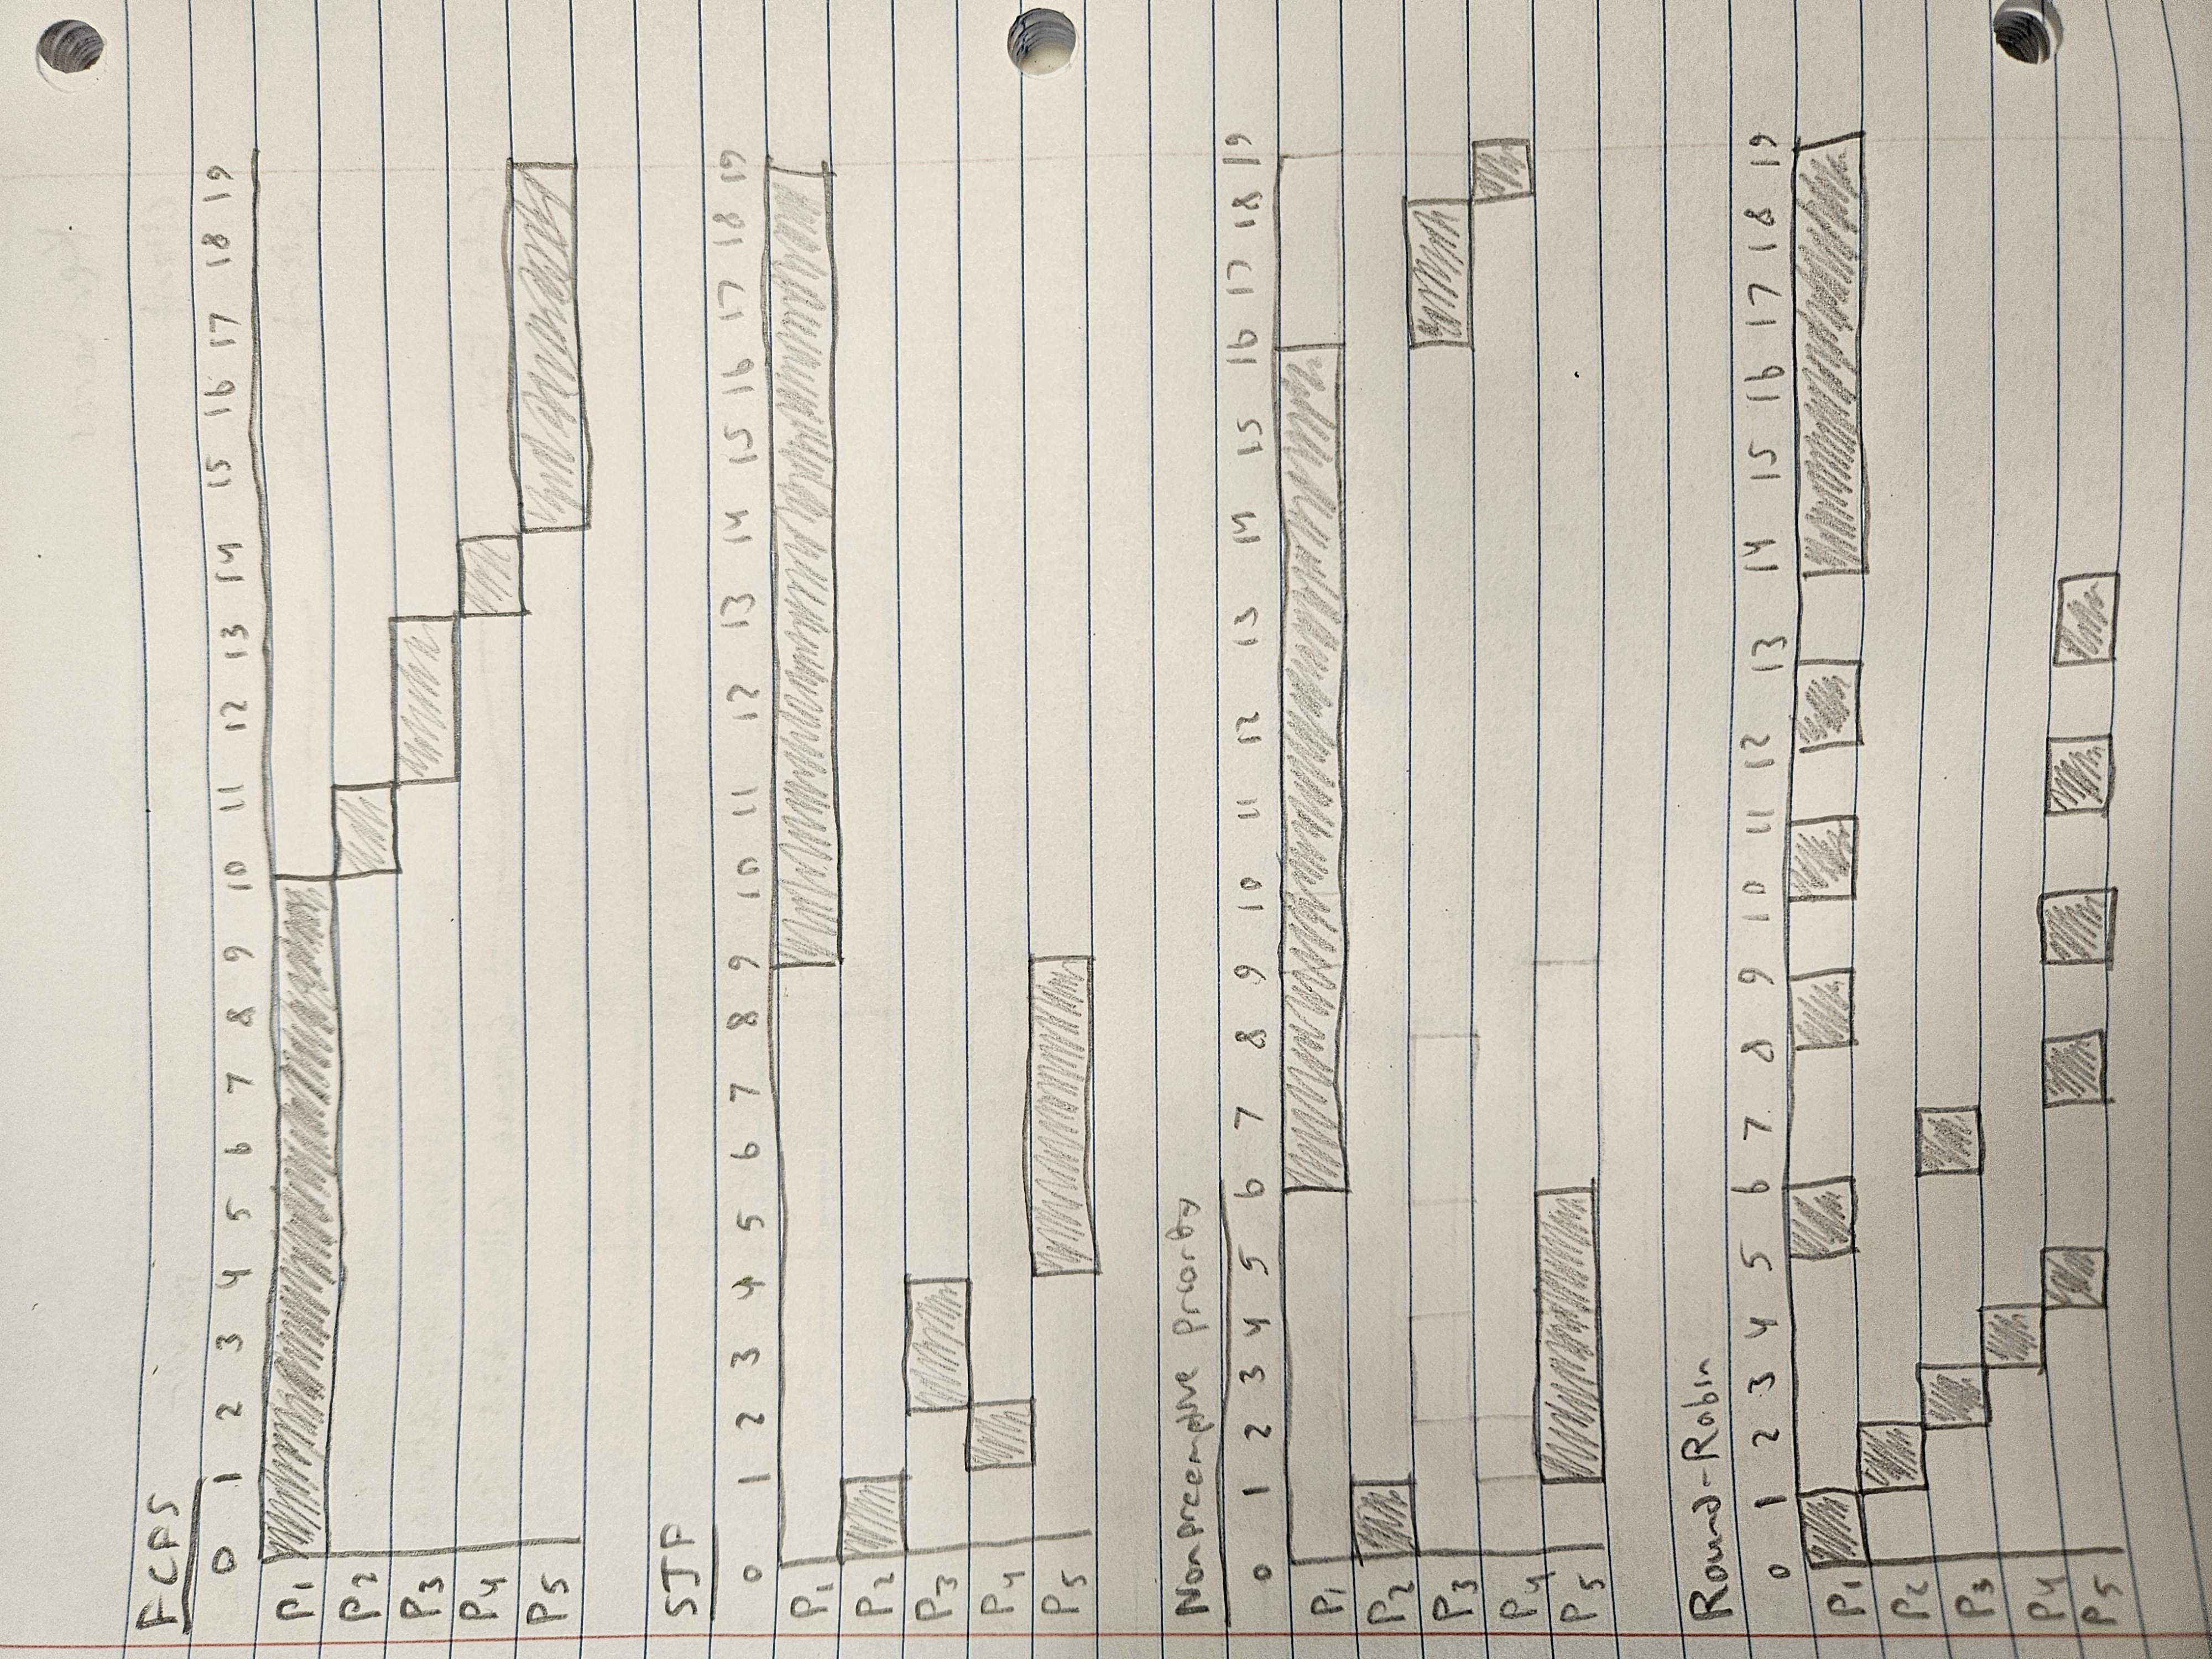
\includegraphics[width=\textwidth, angle=-90]{gantt_charts.jpg}
\end{center}

\section*{b) Turnaround Time and Waiting Time Table}
All times are in ms.

\begin{center}
\begin{tabular}{|c|c|c|c|c|c|}
\hline
Algorithm & Process & Burst Time & Turnaround Time & Waiting Time & Average Waiting Time \\
\hline
\multirow{5}{*}{FCFS} & $P_1$ & 10 & 10 & 0 & \multirow{5}{*}{9.6} \\
& $P_2$ & 1 & 11 & 10 & \\
& $P_3$ & 2 & 13 & 11 & \\
& $P_4$ & 1 & 14 & 13 & \\
& $P_5$ & 5 & 19 & 14 & \\
\hline
\multirow{5}{*}{SJF} & $P_1$ & 10 & 19 & 9 & \multirow{5}{*}{3.2} \\
& $P_2$ & 1 & 1 & 0 & \\
& $P_3$ & 2 & 4 & 2 & \\
& $P_4$ & 1 & 2 & 1 & \\
& $P_5$ & 5 & 9 & 4 & \\
\hline
\multirow{5}{*}{Priority} & $P_1$ & 10 & 16 & 6 & \multirow{5}{*}{8.2} \\
& $P_2$ & 1 & 1 & 0 & \\
& $P_3$ & 2 & 18 & 16 & \\
& $P_4$ & 1 & 19 & 18 & \\
& $P_5$ & 5 & 6 & 1 & \\
\hline
\multirow{5}{*}{Round Robin} & $P_1$ & 10 & 19 & 9 & \multirow{5}{*}{5.4} \\
& $P_2$ & 1 & 2 & 1 & \\
& $P_3$ & 2 & 7 & 5 & \\
& $P_4$ & 1 & 4 & 3 & \\
& $P_5$ & 5 & 14 & 9 & \\
\hline
\end{tabular}
\end{center}
Shortest Job First has the shortest wait time in this scenario.

\end{document}